% Developed architecture / system design / implementation:
% start with a theoretical approach
% describe the developed system/algorithm/method from a high-level point of view
% go ahead in presenting your developments in more detail

\chapter{\project's Design}\label{ch:design}\glsresetall
% Our application is building entirely on decision making. If it seems like a \ac{pd} is coming up, buy, then sell on profit. Otherwise, wait for a \ac{pd}. Simple, yet effective if and only if the application can make accurate predictions. Our prediction algorithm needs to either detect \acp{pd} before it happens or exactly when it begins, because of the period where \ac{pd} peak span from seconds to max $10$ minutes as described in \autoref{sec:pd}. Are we too late with buying assets we may end up buying at or right before the peak which will result in a substantial loss because of the forthcoming dump. However, if we can manage to purchase assets just a few seconds in or before the \ac{pd} starts we can profit well by selling only a short time later when the coin peaks.

% For the application to have the ability to make accurate predictions, we need to carefully define a suitable algorithmic model that fits currently existing data to reverse engineer \acp{pd}. We find two paradigms \emph{financial} and \emph{\ac{ml}} as appealing fields for finding suitable algorithmic models. We encounter some problems in the field of finance, typically, financial institutions do not share their algorithms for competitive reasons, and we can not either find any models that are compatible for detecting \ac{pd} in real-time on cryptocurrency exchanges. We believe that using \ac{ml} to detect \acp{pd} is currently the optimal solution, and to reinforce that assumption, a recent PwC\footnote{Price Waterhouse Coopers is the largest network of accountants, lawyers and advisors, and deliver services within audit, consulting and tax.} study found that over the next two to three years \ac{ml} are the single most crucial technology impacting the finance function~\cite{pwc} as \ac{ml} models seem to excel financial models.


% Supervised learning problem
% binary classification problem
% Pump are anomalies
% choosing a model

% Moving on with \ac{ml}, we can define detection of \ac{pd} as a supervised \emph{binary classification} problem, \ac{pd} or not \ac{pd}. As with every supervised problem we need data that is labeled which are struggling to get.


% Our application only requires the knowledge of the pump part in a \ac{pd} to function. Our application wants to buy before or at the beginning of a pump and sell when the coin peak.

% Our application only requires the knowledge of the pump part in a \ac{pd}, as our application want to buy before or at the beginning of a pump and sell when the coin peak. We can ignore the dump part because it do not affect the decision made by our application. We can define this as a \emph{binary classification} problem, pump or not pump, or from our application perspective buy or sell.

% \acp{pd} are a common price manipulation scheme one observe on cryptocurrency exchanges, but in vast amount of existing data that exchanges produce a \ac{pd} is an \emph{anomaly}. It exist way more regular data than \ac{pd} data. This becomes problem when we want to  create a dataset containing regular data and \ac{pd} data because of the huge imbalance between the two classes, and \acp{pd} are rare entities hence it is also challenging to obtain a significant amount of \acp{pd} required to train a \ac{ml} model.

% Choosing a \ac{ml} model primarily depends on the nature of the input data. Input data can be broadly classified into sequential (e.g., voice, text, music, time series, protein sequences) or non-sequential data (e.g., images, other data)~\cite{dl_anomaly}. Cryptocurrency sources produce sequential data, more specifically \emph{time series} data. Time series data are linearly ordered sequence of values of a variable at equally spaced time intervals~\cite{stat_handbook}. 

% Anomaly detection in sequential data has attracted significant interest in the literature due to its applications in a wide range of engineering problems. \ac{lstm} neural network based algorithms for anomaly detection have been investigated and reported to produce significant performance gains over conventional methods  (Ergenet al. [2017]).

% Supervised anomaly detection techniques are superior in performance compared to unsupervised anomaly detection techniques since these techniques use labeled samples (G ̈ornitz et al. [2013]).  Supervised anomaly detection learnsthe separating boundary from a set of annotated data instances (training) and then, classify a test instance into eithernormal or anomalous classes with the learned model (testing).

% Moreover, the performance of deep supervised classifier used an anomaly detector is sub-optimal due to class imbalance (the total number of positive class instances are far more than the total number of negative class of data)~\cite{dl_anomaly}.

% Labels indicate whether a chosen data instance is normal or an outlier. Anomalies are rare entities hence it is challenging to obtain their labels~\cite{dl_anomaly}.
TBW
\section{Overview}
We are modeling \project as a \ac{ml} pipeline, but with some few extensions. It is designed to extract raw data from different cryptocurrency sources and transform it into valuable features in order to classify \acp{pd}. The term \ac{ml} pipeline can be misleading as it implies a one-way flow of data when some elements in the pipeline are cyclical and iterative where every iteration intends to improve the accuracy of the model~\cite{ml_pipeline_3}. Some of the advantages a pipeline provides is~\cite{ml_pipeline_2};

\begin{itemize}
    \item \textbf{Flexibility} - Processing elements are easy to replace and to modify without changing the system.
    \item \textbf{Extensibility} - The system is partitioned into pieces making it easy to add new functionality.
    \item \textbf{Scalability} – Each processing element is separately scalable because they are independent.
\end{itemize}

\begin{figure}[ht]
    \centering
    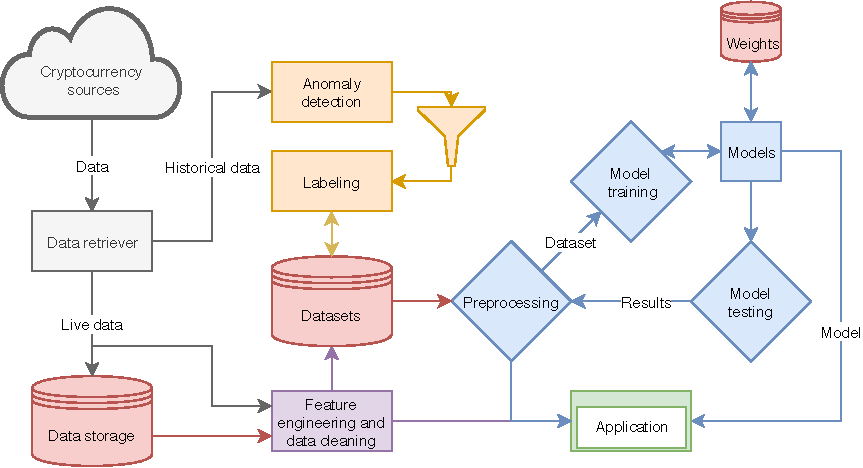
\includegraphics[width=\textwidth]{overview.pdf}
    \caption{Architectural overview of \project}
    \label{fig:overview}
\end{figure}

The first step in the pipeline pulls data from various cryptocurrency sources. The data is mostly incomplete and lacks behaviors or trends making it currently pointless to train a model with. This process is tedious because sources tend to have different request rates, \acp{api}, and the data can have various formats like \ac{json} or \ac{xml}.

The next step branches the retrieved data in two, live and historical data. Since we are trying to detect \acp{pd} in real-time we need to store live data continuously. When captured a compelling amount of \acp{pd} in the stored live data, we use an anomaly detection algorithm~\cite{P&D_to_the_moon} to detect \ac{pd} in the gathered live data. This algorithm is not compliant with live data, so we need to pull aggregated historical data that span throughout the collected live data. As previously mentioned, anomaly detection algorithms tend to have a high false positive rate. Thus, we need to remove these false positive and keep the true positive manually.

The input data ultimately determine the performance of a \ac{ml} deep learning model~\cite{mike_voets}, so training a model with the raw gathered live data is ineffective. Hence, we need to define new convenient dataset containing features created by processing the collected live data; this is a highly critical process and will later determine the classification performance of the deep learning model. The gathered live data also need to go through a cleansing process as it most likely does not contains relevant \ac{pd} information.

With filtered anomalies containing \ac{pd} and a dataset, we can create a labeled dataset and train our model. Obtaining good classification results depends, as mentioned, on the features, but also how we decide to pre-process the dataset. Typical pre-processing strategies include dimensionality reduction and normalization. Having a labeled pre-processed dataset we can finally begin to the train the deep learning model, this a cyclical and a long process, as it requires many trial and error attempts to find the optimal weights for the model. In each cycle, we store the model's weights because it is not always the case that each iteration will improve the classification performance of the model.

For applications to utilize \project, they need to select a model and let live data flow through the same processing stages as the dataset that was used to train the model.

\section{Internal Components}
TBW

\subsection{Retrieving Data}
Every problem that is solved using \ac{ml} requires data, the more, the merrier when training a model. As previously mentioned, cryptocurrency sources like exchanges produce time series data containing, e.g., price and volume of a coin. Such data is continuously produced in a restricted amount with proportion to time.

Since we want to detect \acp{pd} on exchanges in real-time, the nature of the data we want to make classifications on is  live fine-grained data so that the model can detect them as early and accurate as possible. Aggregated historical data is too coarse-grained because exchanges generally only allow a discrete time interval selection of data where the smallest is typically one minute. The duration where they start to where they peaks varies from a few seconds to max ten minutes~\cite{P&D_MIT_crypto, P&D_to_the_moon}, and the ability to make accurate predictions with one-minute data is questionable.

Training a model in real-time by pulling data is impractical because we do not have the \acp{pd} labels then, and sources can only produce a limited amount of data at a time which will create a bottleneck of data supply to the model. To cope with these problems, we have to pull and store current live data continuously; this is an endless dreary process for we have to wait weeks until we have "captured" enough \ac{pd} events in our collected data to start training. If anything fails, we may have to start all over again as we are missing out on trends, which results in noisy data.

From the reinforcers field in \autoref{tab:pd_indicators}, to reverse engineer \acp{pd}, we have to fetch data from various sources. An exchange alone does not produce data regarding a coin's capitalization, nor a coin's price on a different exchange. Other sources than exchanges produce such metadata of coins, while exchanges only produce internal trading data.

\subsubsection{Master Slave Approach}
We shape our data retriever like a \ac{ms} model. The term \ac{ms} is through a quiet ongoing debate in the coding community~\cite{giz_master, reg_master, med_master}, as some may interpret it offensively and relate to the institution of slavery. Our intention is not to insult anyone, but we are still using this term because none have yet proposed a lasting substitution to it.

\begin{figure}[ht]
    \centering
    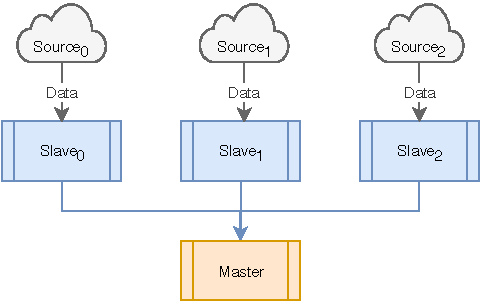
\includegraphics[width=0.8\textwidth]{ms.pdf}
    \caption{\acf{ms} structure}
    \label{fig:ms}
\end{figure}

Nevertheless, In computing networking, \ac{ms} is a model for a communication protocol in which one process (master) controls one or more processes (slaves)~\cite{ms_bs}. \autoref{fig:ms} is an example that illustrates our data retriever with a master and its three data pulling slaves. Each slave in our data retriever is assigned a source that can be, e.g., an exchange. The communication between slaves and the master is intuitive. The master broadcasts a pull signal to the slaves, and they pull the data from their assigned source, then the master gathers the data from them and parses it, and augments it to a sample. Each sample the master generate gets stored. This procedure takes effect in a fixed interval for obtaining clean time series data, such that each sample's time gap is equal. The advantages and disadvantages of this structure are:

\textbf{Advantages}
\begin{enumerate}
    \item \emph{asynchronous requests} - Each pull-broadcast issued by the master starts a series of requests in parallel from the slaves. Thus, each request is roughly issued simultaneously making features in a sample equally spaced in terms of time.
    % Frequently fetching of data from the internet is an \ac{io} bound problem, and are typically solved with multiprocessing or concurrency if needed. If we choose a single process to make synchronous requests, a bottleneck could have occurred, and requests would be issued separately that results in various time gap among features in each sample.
    
    \item \emph{removes race condition} - Since each data sample is \emph{sequentially} written to disk by the master, a race condition can not take place. 
    % If the slaves processed their data and wrote to the same location, at some point in time, a race condition would take place and corrupt the data. Even though these race conditions are rare, anything that can happen will happen, Murphy's law.
    
    \item \emph{horizontal scaling} - Scales by adding slaves instances~\cite{ms_hor}; there is no upper limit of them. In the end, the bottleneck is the master if its have too many of them to communicate with.
    
    \item \emph{faulty slave tolerance} - If a slave crash, the data retriever is still progressing, but it also results in partial storage of data. Hence, this will most likely corrupt a good portion of the collected data.
\end{enumerate}

\textbf{Disadvantages}
\begin{enumerate}
    \item \emph{\ac{spof}} - If the master crash, the slaves will not retrieve data.
\end{enumerate}

\subsubsection{Collecting Trading Data From Multiple Markets}
Previous work in detection of \acp{pd}~\cite{P&D_to_the_moon}, estimated that $1.6$ \acp{pd} is carried out daily per market, this raises several problems. First, multiple exchanges have the same market, and we can not know which exchange they target unless we have prior knowledge from their \ac{pd} group. Second, gathering data from a single market is inadequate, the data retriever would with an estimate captured $48$ \ac{pd} occurrences, if it gathered every \ac{pd} event on a single market in a whole month. Training a model with $48$ instances is insufficient. 

Therefore, we collect data from all the markets from a single exchange to make sure we obtain as many \acp{pd} as possible. Inbefore doing that, we need to make a considerable assumption, that is, \acp{pd} pattern remain the same across markets. Otherwise, if it does not, we may run into trouble when training our model by having too few samples with various patterns. By training a model using data from all the market makes it general, allowing it to adapt to new markets as the exchange issues them. 

The reason we are targeting a single exchange is that they have different \acp{api}, although the data they provide are mostly identical, in some way, each exchange does stand out by providing some unique data. Thus, we can utilize every piece of information we receive from an exchange without the concern of making it compatible with data existing on other exchanges.

\subsubsection{Feature Description}
From the \ac{pd} indicators described in \autoref{tab:pd_indicators}, we define a set of features described in \autoref{tab:features}, we believe that these features contains the necessary information for a model to detect \acp{pd}. We fetch all these features for each market.

Some features like a coin's capitalization are available at \href{https://coinmarketcap.com/}{CoinMarketCap}, while trading data like order book and \ac{ohlcv} values are available at exchanges. A specific feature that is challenging to attain is aggregated \ac{ohlc} values from multiple exchanges, as this requires us to request multiple exchanges simultaneously and aggregate the data.

\begin{table}[ht]
    \centering
    \begin{tabular}{p{0.30\textwidth} p{0.70\textwidth}}
        \hline
        \textbf{Feature} & \textbf{Description}\\
        \hline
        \ac{ohlcv}                      & Latest \ac{ohlcv} values.\\
        \hline
        \ac{ohlcv} multiple exchanges   & Aggregated \ac{ohlcv} values from multiple exchanges.\\
        \hline
        Order book                      & Level $1$ (aggregated price and volume) order book with a depth of $5$.\\
        \hline
        Order book imbalance            & The imbalance between bids and asks orders and quantity.\\
        \hline
        Coin capitalization ratio       & Coin capitalization ratio.\\
        \hline
        Volume traded                   & Base and quote volume traded for the last $24$ hours.\\
        \hline
        number of trades                & Number of completed trades for the last $24$ hours.\\      
        \hline
        bid and ask price               & Best bid and ask price for the last $24$ hours.\\
        \hline
        bid and ask volume              & Best bid and ask quantity for the last $24$ hours.\\
        \hline
        Average price                   & Average price for the last $24$ hours.\\
        \hline
        symbol-pair exchange rate       & The rate of how many exchanges that lists the symbol-pair.\\ 
        \hline
        Time                            & Unix timestamp.\\
        \hline
    \end{tabular}
    \caption[Features description]{Feature description}
    \label{tab:features}
\end{table}


\newpage
\subsection{Preparing Data}\label{sec:prep}
In practice, it has shown that data cleaning and preparation takes approximately $80\%$ of the total data engineering effort, as it requires solid domain knowledge of the subject. Data preparation is, therefore, an important research topic. Data preparation comprises those techniques concerned with analyzing raw data to yield quality data, mainly including data collecting, data integration, data transformation, data cleaning, data reduction, and data discretization~\cite{zhang2003data}.

For the reason that we fetch data from multiple sources and markets to create a general model, we must prepare the data for it. Since markets are distinct, they surely have various numerical values, such as different trading price and volume, and making predictions with these numerical values that fluctuate from market to market is nonviable. E.g., assume a \ac{pd} occurs on a coin with a low cost, and the price is increasing with $300\%$. Despite the high increase and profit, the coin is still almost worthless compared to other expensive coins, and the model do not distinguish between markets, all markets are equally weighted. It looks at each feature as "more" or "less" of something. Thus, we must transform all these numerical values into some other values.

\subsubsection{Data Cleansing}
Data cleaning, also called data \emph{cleansing} or \emph{scrubbing} deals with detecting and removing errors, inconsistencies, and unproductive features from data in order to improve the quality of data~\cite{data_cleaning}.

Fetched data from exchanges includes additional features not defined in \autoref{tab:features}. These features do we have to remove as they probably adds nothing of valuable knowledge. Instead, they increase the number of dimensions and makes the data more complex.

Markets with little or no activity may have intervals containing \emph{zero-data}, e.g., if no investors have bought or sold assets in a specific interval, exchanges tend to set the trading values to zero. These zero-values create significant jumps/spikes in the trend which we must fix; otherwise, they disrupt the data. Besides, having zero-data does not make any sense, if the price is recorded to be zero, then it means that coin is free which it is not.

We substitute every value that is zero by linear interpolate each of them. Linear interpolation involves estimating a new value by connecting two adjacent known parameters with a straight line~\cite{interpolate}. These two known parameters are non-zero values that are adjacent on each side of the zero-value. Thus, we form the following \autoref{eq:interpolation} with the known parameters $(x_1, y_1)$ (previous non-zero value) and $(x_2, y_2)$ (next non-zero value), $y$ is the new value for some zero-value in point $x$.

\begin{align}\label{eq:interpolation}
    y = y_1 + (x - x_1) \frac{y_2 - y_1}{x_2-x_1}
\end{align}

\subsubsection{Feature Engineering}
Feature engineering is the process of using domain knowledge of the data to create features that make \ac{ml} algorithms work. Feature engineering is fundamental to the application of machine learning and is both challenging and expensive, but when done correctly, it can result in wonders~\cite{feature_engin}.

\begin{displayquote}
    \begin{em}
        "Feature engineering is the art part of computer science" - Sergey Yurgenson
    \end{em}
\end{displayquote}
 
\subsubsection{Processing Order Book}
As previously mentioned in \autoref{sec:pump_groups}, \ac{pd} organizers invests in the market before the \ac{pd} without raising the price. We believe that the order book in said market oscillates in before the pump, and especially during the pump. Therefore, we calculate an imbalance between sell and bids order; this is a multidimensional problem considering an order book contains both a list with prices along with its volume as we saw in \autoref{tab:order_book}. \autoref{eq:imbalance} reduces this multidimensional problem to a single value with equal weight to price and volume. $p$ and $v$ is respectively the lists with prices and volumes, and the annotations $a$ and $b$ denotes asks and bids orders. If \autoref{eq:imbalance} yields a value between $(0,1)$, then it weigh more bidders, if it yields a value between $(1, \infty]$, then askers, and $1$, there is an equal weight of bidders and askers.

\begin{align}\label{eq:imbalance}
    imbalance = 
    \frac{
    \begin{bmatrix}
        p^a_1 \\
        \vdots \\
        p^a_n
    \end{bmatrix}
    \cdot
    \begin{bmatrix}
        v^a_1 \dots v^a_n
    \end{bmatrix}
    }{
    \begin{bmatrix}
        p^b_1 \\
        \vdots \\
        p^b_n
    \end{bmatrix}
    \cdot
    \begin{bmatrix}
        v^b_1 \dots v^b_n
    \end{bmatrix}
    }
    = \frac{\langle P_a, V_a \rangle}{\langle P_b, V_b \rangle}
\end{align}

\subsubsection{Processing Trading Data}
We process trading data such as price and volume by calculating the percentages of change, which makes each market comparable and eliminates the need for the model to adjust to prices. For example, if ETH is up \$$10$ from a starting value of \$$100$, and ADA is up \$$5$ from a starting value of \$$50$, then both coins are up $10$\%.

We define the function $pct$ to calculate the percentage of change. It calculates the percentage change in point $x$ concerning a previous value $v$ with a time lag $\gamma$. We consider $x$ and $v$ to be a single value like the price or volume, while $\gamma$ indicates moving backward in time from point $x$. We must be vigilant when using this technique, if the data contains values that are zero, we might perform a zero-division that can clutter with the data unpredictably. However, since we scrubbed the data first and removed this zero-values, this should not be a concern.

\begin{align*}%\label{eq:pct}
    pct(x, v_\gamma) = \frac{x - v_\gamma}{x}
\end{align*}

Differentiating and take the tangent line instead could be a solution, but since we are fetching data from multiple markets, the tangent would always favor expensive markets. Using the tangent would be illogical when \ac{pd} organizers tend to target low-cost markets.

\subsubsection{Processing Time}
According to \cite{P&D_anatomy}, the time is essential when classifying \acp{pd}, as they are typically executed at the hour (6:00, 7:00, etc.) because organizers usually does not choose a random time.

\begin{equation}\label{eq:unix_time}
    x_\delta(x_{\textbf{unix}}) = \frac{x_\textbf{unix}\mod 3600}{3600}
\end{equation}
\myequations{UNIX timestamp scaling}

\begin{align}\label{eq:gaus}
    t(x_\delta, \mu, \sigma) &= \frac{1}{\sqrt{2\pi\sigma^2}} e^{-\frac{x_\delta-\mu}{2\sigma^2}}, \quad \text{where}
    \begin{cases}
    \mu = 0.5 \\
    \sigma = 0.1 
    \end{cases}
\end{align}
\myequations{Data preparation - Time}

Data retrieved from sources are getting timestamped, and we can take advantage of these timestamps to check whether data was generated at the hour or not. The function $x_\delta$ transforms a Unix\footnote{unix timestamp is a way to track time as a running total of seconds.} timestamp to a value in the interval $[0, 1)$. The closer $x_\delta$ is to the margins, the closer the time is at the hour, but since $0$ and $1$ symbolizes the same, we have to process it further before we can use it as a valuable feature.

We define a Gaussian distribution function $t$ with the parameters $\mu=0.5$ and $\sigma=0.1$ which creates the graph illustrated in \autoref{fig:unixtime}. The graph shows when given $t$ a $x_\delta$ close to $0$ or $1$ (6:00, 7:00, etc.), $t$ returns a value close to $0$, but when given $0.5$ (6:30, 7:30, etc.) it returns a value close to $4$. $t$ demonstrate that we can separate data by how close it was generated at the hour. Also, we can always tweak $\sigma$ to adjust the width of the wave. Adjusting the wave allows us to be more strict, the wider the curve, the more strict.

\begin{figure}
    \centering
    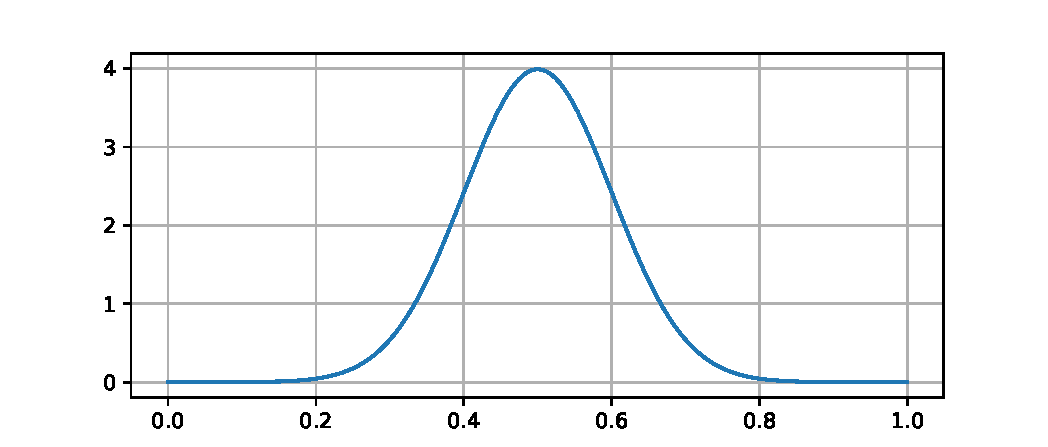
\includegraphics[width=\textwidth]{time.pdf}
    \caption{Gaussian distribution}
    \label{fig:unixtime}
\end{figure}

\subsection{Collecting Pump-and-Dumps}
Manually collecting \ac{pd} events from chat applications to label our collected data, seems infeasible in the long run — even tough Livshits and Xu \cite{P&D_anatomy} hand-picked $220$ pump-events from July to November in 2018 from $358$ different Telegram groups to train a Random Forest. They still did miss out on plenty of other executed \ac{pd} schemes as there are numerous of other chatting applications and private organizers~\cite{blockonomi}. Also, searching for \ac{pd} events is a time-consuming process, and incorrect labeling occurs when we lack membership to all of \ac{pd} groups, which results in more mediocre prediction capacity~\cite{label_noise}. We also have to be aware if a \ac{pd} was successfully executed or not; labeling failed attempts as positive only contributes to label noise. Instead of manually collecting \acp{pd} from groups in chatting applications, we believe that it is possible to hand-pick \acp{pd} by \emph{reasoning abductively} with the help of an anomaly detection algorithm to pinpoint suspicious time intervals in historical data.

The anomaly detection algorithm identifies local \emph{contextual anomalies} based on fixed recent history called a \emph{sliding time window}. Contextual or conditional anomalies are abnormal data points within a specific context and are prevalent in linearly ordered data called \emph{sequence data}~\cite{anomaly_survey}. A sliding window is a period that stretches back in time (lag factor) from the present containing events at specified intervals. The event intervals can overlap with each other, or they can be disjunct. As events exceed the lag factor, they fall out of the sliding window, and they are no longer matching against the rules applied to the sliding window~\cite{redhat}. With a sliding window, we can compare values in a given period~\cite{P&D_to_the_moon}, contrary to using single values, which not yield much information alone in sequence data.

The anomaly detection algorithm is proposed by Kleinberg and Kamps \cite{P&D_to_the_moon}, which is inspired by previous research in \ac{dos} attacks~\cite{dos}. It is a threshold based technique to find a suspicious increase in price and volume of a coin. If the price and volume in a specific interval are higher than some threshold, then the interval is flagged anomalous and worth further investigation.

\subsubsection{Price Anomaly}
We compute the price anomaly threshold by a simple moving average $\mu_\gamma^p$ of \ac{ohlcv} values denoted $x$ with a lag factor $\gamma$ multiplied with a given percentage increase $\epsilon_p$. We consider $x$ and $\gamma$ as \ac{ohlcv} objects, and $x-\gamma$ indicates moving backwards in the sliding time window by a factor of $\gamma$~\cite{P&D_to_the_moon}. If the highest registered price in $x$'s period is greater than the computed threshold, we flag the period as anomalous.
\begin{align}
    \mu_\gamma^p(x) &= \frac{\sum^x_{i=x-\gamma} x_{close}}{\gamma}\\
    price\_anomaly(x)&=
    \begin{cases}
        True  & \text{if $x_{high} >    \epsilon_p \cdot \mu_\gamma^p(x)$}\\
        False & \text{otherwise}
    \end{cases}
\end{align}

\subsubsection{Volume Anomaly}
Calculating the volume anomaly threshold is almost identical to the above, we are only substituting $x_{closing}$ and $x_{high}$ with $x_{volume}$, which form the following expression.
\begin{align*}
    \mu_\gamma^v(x) &= \frac{\sum^x_{i=x-\gamma} x_{volume}}{\gamma}\\
    volume\_anomaly(x)&=
    \begin{cases}
        True  & \text{if $x_{volume} >    \epsilon_v \cdot \mu_\gamma^v(x)$}\\
        False & \text{otherwise}
    \end{cases}
\end{align*}
\myequations{Anomaly - Volume}

\subsubsection{Filtering Anomalies}
Anomaly detection algorithms, in overall, have a high false alarm rate~\cite{grill2017reducing}, which makes them difficult to use. Since we want to use these anomalies we collected to train a model with, it is, with high importance, to remove false \acp{pd}. Otherwise, training a model with false \acp{pd} will make the model perform worse, and results in a high occurrence of false positives which is already a problem. Therefore, we manually remove all the false positives anomalies, but removing them requires prior knowledge of \acp{pd}, which we do not have.

Since the anomaly detection algorithm checks whether a \ac{pd} occurred in a specific interval, and not exactly when. We visualize one-minute \ac{ohlc} from that interval in a chart, by plotting these values we can compare them to a few charts containing real \ac{pd}. Additionally, a market's capitalization, if the pairing coin is BTC, or how many exchanges that list the market, can be helpful when filtering \ac{pd}. E.g., if the anomaly detection algorithm flagged a suspicious interval in the ETH-BTC market, and it visually looks like a \ac{pd}, then it still would with a high likelihood not be a \ac{pd} because ETH is the coin with second highest capitalization~\cite{coinmarketcap_eth}, and that would break the pattern where the organizers target coin with low capitalization. Further helpful characteristics regarding \acp{pd} is described in \autoref{tab:pd_characteristics} and \autoref{tab:pd_indicators}.

\subsubsection{Labeling Pump-And-Dumps}
With the new features generated by the collected data and filtered anomalies containing \acp{pd}, we can label the new features and define a dataset, but first, the filtered anomalies still contains intervals where \acp{pd} occurred, and not exactly when it was executed. So, we need to precisely define where every \ac{pd} started end ended, before labeling.

Because the purpose of \acp{pd} is to raise the price of an asset, makes us believe that, where the price change is highest in an interval, that is where the \ac{pd} peaked. If we have the peak of a \ac{pd}, we can search from the peak and down the descending slopes on each side of it. Left side, pump. Right side, dump. From each side we search until the change in price is equal or smaller than $0$. Finally, when have defined the start and end of every \ac{pd}, we label all the new features positive where there are \acp{pd}, and negative otherwise.

\subsection{Deep Learning}
This section describes the model we use to detect \ac{pd}, and how we process data, trains the model, and which metrics we should use to evaluate the model. These steps are an iterative process, where each iteration tend to improve the model.

\subsubsection{Preprocessing}
Before training a model with the generated dataset, we transform it by \emph{normalizing} Since the features in our dataset have various scales, some percentages, some other numerical values, then, a common technique do is to \emph{normalize} the input data. Normalization creates new values from the dataset, but still maintain the general distribution and ratios in the source data while keeping values within a scale applied across all used features~\cite{normalize_data}. Also, normalization, in some cases, improves the performance of the model~\cite{normalize_google}, and accelerate convergence speed resulting in shorter training time~\cite{sola1997importance}.

There are several ways to normalize data, and which normalization technique one use may have an impact on the performance of the model. Since \acp{pd} are anomalies, some features like percentage change in price and volume will make them look like outliers in the data. A traditional method called \emph{min-max} normalization is repeatedly used in detection of outliers~\cite{campos2016evaluation, goldstein2016comparative}. This technique provides a linear transformation of the data~\cite{panda2014smoothing}, allowing us to keep the distance ratio, and it scales every value into the range $[0,1]$.

\begin{align}\label{eq:minmax}
    x_{ij}' = \frac{x_{ij} - \min(x_j)}{\max(x_j)-\min(x_j)} 
\end{align}

\autoref{eq:minmax} is the min-max normalization formula for a coefficient $x_{ij}$, where $x_j$ is a column in a dataset with row vectors.

\subsubsection{Model}
The basic model type we use to detect \ac{pd} is a \ac{rnn} \ac{lstm} network. This network contains \ac{lstm} cells in the hidden layer because we want the cells to have an internal state (memory) to remember the trend in data. We modeled the detection of \acp{pd} as \emph{binary classification} problem, \ac{pd} or not \ac{pd}. So, we only need a single perceptron in the output layer. \autoref{fig:lstm} illustrates the model.

We can build a more complex network with multiple layers containing \ac{lstm} and perceptron cells, but with a deeper network, the time it takes to train increases simultaneously as it is harder to find the optimal parameters of the network. 

\begin{figure}[ht]
    \centering
    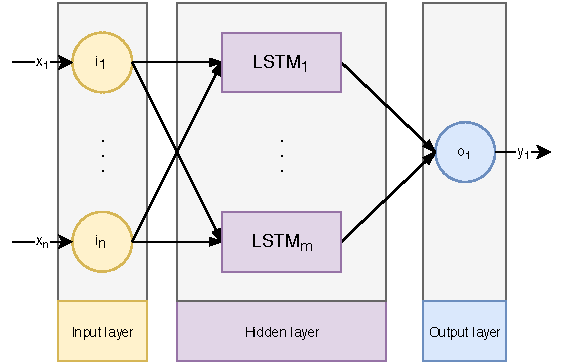
\includegraphics{lstm.pdf}
    \caption{Structure of the model}
    \label{fig:lstm}
\end{figure}

\subsubsection{Training}
Before we start to train our model, we have to split the dataset into two sets, a training set, and a test set. The training set will we use to train the model, and the test will we use to evaluate the model. There is also a validation set that is used to fine-tune the hyperparameters during the training, but since there are so few \ac{pd} samples, we choose to avoid using a validation set and use those \ac{pd} samples we have to train our model and evaluate it.

As previously mentioned, \acp{pd} are anomalies, and that results in a significant class imbalance between positive and negative samples, which, when trained will make the model to overfit to the negative class and more or less ignore the positive class, it entirely depends on the distribution of them. Also, the academia is split concerning the definition, implication and possible solutions to this problem~\cite{tw_imbalance_2} making it currently ambiguous how to properly deal with it.

\begin{figure}[ht]
    \centering
    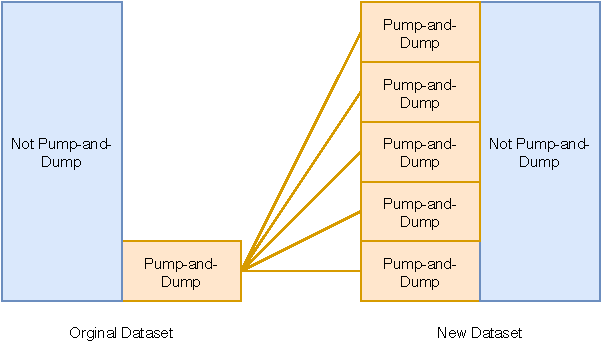
\includegraphics{oversampling.pdf}
    \caption{Oversampling (source\cite{tw_imbalance})}
    \label{fig:oversampling}
\end{figure}

We believe that we can solve our imbalance problem by using a technique called \emph{oversampling}, which \autoref{fig:oversampling} illustrates. Oversampling gathers all the samples from the minority class and duplicates them until the amount is approximately equal to the majority class. There is also a technique called \emph{undersampling}, that select random samples into a subset from the majority class until the size is equal to the number of samples in the minority class, but by using the oversampling technique, we can train our model with the whole dataset. With a balanced dataset, we can finally train our model.

Sometimes, depending on the size of the dataset and number of epochs, training a model takes a really long time. Thus, after each training, we store the model and all its weights and other internal parameters.

\subsubsection{Evaluation}
After the training phase, we evaluate the model by classifying all the samples in the test dataset. The metrics, \emph{precision}, \emph{tp-rate}, and \emph{fp-rate} are probably the most important metrics to optimize when it comes to detection of anomalies. Sometimes, finding the best parameters is done by multiple trials and errors attempts. Adjusting the parameters like number of, hidden layers, cells, and epochs, might improve said metrics. Also, shuffling samples may improve the model as we train with a few numbers of original \acp{pd} samples.

\section{Stitching it all together}
Till now, in this chapter, we have described each component in \project. As we mentioned in \autoref{ch:background}, when we have trained a model and are satisfied with how it performs, we can be fed the model with real-time data, and it will classify whether the given data is a \ac{pd} or not. This allows us to dismiss numerous components which are not needed anymore. They only need to be present during the training phase. So we can divide \project into two phases, a training phase, and a deployment phase. In the training phase, \project entirely depends on all the components. In the deployment phase, there are only a few necessary components.

\subsection{Deployment Phase}
In the deployment phase, we only need a handful component, these components are in \autoref{fig:pipe}. The first component, the retriever function precisely like described above, it fetched data and pushes it further down the pipeline, but it is essential that it fetches the same type of data from the same sources. The next two stages are different, as they need to remain a state from the training phase. In the feature engineering stage, we have to use the same parameters in the cleansing and feature engineering method. Otherwise, the model will classify data that is not what it trained with. Also, in the processing stage, it is highly essential that we normalize the input data with the precisely same parameters as we used with the training set. Else, the input data is scaled the inconsistent parameters, which with result in more misclassification.

The application needs to select a model that was generated during the training phase. With both a trained model and processed real-time data, the application can with ease predict in real-time, whether if the input data is a \ac{pd} or not.

\begin{figure}[h]
    \centering
    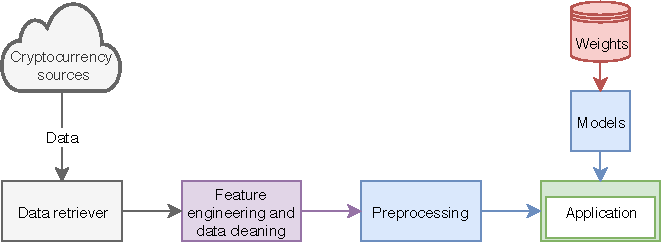
\includegraphics{pipe.pdf}
    \caption{Deployment pipeline}
    \label{fig:pipe}
\end{figure}